\begin{center}
\footnotesize\noindent\fbox{
	\parbox{\textwidth}{
Verificato che la funzione \(f(x_1,x_2) = x_1^2+x_2^3-x_1x_2\) ha un punto di minimo relativo in (1/12, 1/6), costruire una tabella in cui si riportano il numero di iterazioni eseguite, e la norma euclidea dell'ultimo incremento e quella dell'errore con cui viene approssimato il risultato esatto utilizzando la function sviluppata al punto precedente per valori delle tolleranze pari a \(10^{-t}\), con t = 3,6. Utilizzare (1/2, 1/2) come punto di innesco. Verificare che la norma dell'errore \'e molto pi\'u piccola di quella dell'incremento (come mai?)
	}
}\end{center}

\noindent Si verifica innanzitutto analiticamente l'esistenza di un punto di minimo relativo in (1/12, 1/6). Si rinominano le variabili in x ed y per convenienza nella notazione.
\[
\frac{\partial}{\partial x}f(x,y) = 2x -y \quad \frac{\partial}{\partial y}f(x,y) = 3y^2 - x
\]
\noindent Si ottiene il sistema non lineare:
\[
\begin{cases}
2x -y = 0 \\
3y^2 - x = 0
\end{cases}
\quad \text{che ha come soluzioni} \quad x=0, y=0 \quad \text{e} \quad x=\frac{1}{12}, y=\frac{1}{6}
\]
\noindent I punti trovati sono quindi punti stazionari della funzione data.
\[
H =
\begin{bmatrix} f_{xx} & f_{xy} \\ f_{yx} & f_{yy} \end{bmatrix}
=
\begin{bmatrix} 2 & -1 \\ -1 & 6y \end{bmatrix}
\quad
\det(H) = 12y -2
\]

\noindent Il determinante della matrice Hessiana \'e nullo per \(y=\frac{1}{6}\), non si pu\'o concludere ancora niente.

\[
f(\frac{1}{12}, \frac{1}{6}) = -\frac{1}{432} \quad \overline{f}(x,y) = f(x,y) + \frac{1}{432} \quad \overline{f}(\frac{1}{12}, \frac{1}{6}) = 0
\]
\\

\noindent Si studia il segno di \(\overline{f} \) con il seguente codice Matlab:
\\
\lstinputlisting[language=Matlab]{cap3/3_11_sign.m}

\begin{center}
	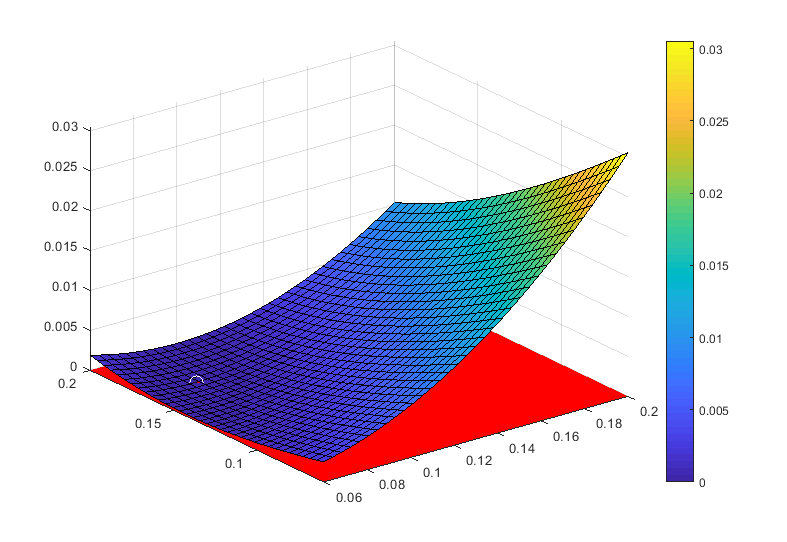
\includegraphics[scale=0.7]{cap3/3_11_sign.png}
\end{center}

\noindent Poich\'e \(\overline{f}\) \'e tutta positiva in un intorno di \((\frac{1}{12}, \frac{1}{6})\), possiamo concludere che quel punto \'e sicuramente un minimo relativo di \(f\).

\noindent Per quanto riguarda l'utilizzo del metodo di Newton, \'e stata scritta una versione modificata della function dell'Esercizio precedente per restituire i dati da mostrare nella tabella richiesta.
\\
\lstinputlisting[language=Matlab]{cap3/3_11.m}

tabella da riempire
\begin{tabular}{l*{15}{c}}
 it. & \vline& \(x_1\) &\vline& \(x_2\) & \vline& appr. \(\sqrt\alpha \) & \(\Delta\sqrt\alpha \) \\
\hline
 1 & \vline& 3      & 0.7639				& \vline& 2.5000 & 0.2639 \\
 2 & \vline& 2.3333 & 0.0973				& \vline& 2.2727 & 0.0367 \\
 3 & \vline& 2.2381 & 0.0020				& \vline& 2.2381 & 0.0020 \\
 4 & \vline& 2.2361 & 9.1814 \(\times10^{-7}\) 	& \vline& 2.2361 & 1.6475 \(\times10^{-5}\) \\
 5 & \vline& ''     & 1.8829 \(\times10^{-13}\)	& \vline& ''     & 7.4651 \(\times10^{-9}\) \\

\end{tabular} \\

% 10^-3 i= 10
% incr 0.00077204
%     "x 0.083577"    "x 0.083577"
%     "x 0.16715"     "x 0.16715"
%
% Minimo :
%     0.0836    0.0836
%     0.1672    0.1672
%
% 10^-4 i=13
% incr 9.6505e-05
%     "x 0.083364"    "x 0.083364"
%     "x 0.16673"     "x 0.16673"
%
%
% 10^-5 i=17
% incr 6.0316e-06
%     "x 0.083335"    "x 0.083335"
%     "x 0.16667"     "x 0.16667"
%
% 10^-6  i=20
% incr 6.0316e-06
%     "x 0.083335"    "x 0.083335"
%     "x 0.16667"     "x 0.16667"

\noindent Come si pu\'o notare, la norma dell'errore...

